\documentclass[upright, contnum]{umemoria}
\depto{DEPARTAMENTO}
\author{AUTOR}
\title{T�tulo}
\auspicio{Conicyt}
\date{A�o}
\guia{Profesor gu�a}
\carrera{MAGISTER}
\memoria{TESIS PARA OPTAR AL GRADO DE}
\comision{Examinador 1}{Examinador 2}{Examinador 3}
 
\usepackage{amsmath}
\usepackage{pdfpages}
\usepackage{amssymb}
\usepackage{color}
\usepackage[latin1]{inputenc}
\usepackage[T1]{fontenc}
\usepackage{physics}
\usepackage{cite}
\usepackage{mathtools}
\usepackage{mathrsfs}
\usepackage{esint}
\usepackage{float}
\usepackage{hyperref}
\hypersetup{
    colorlinks = true,
    allcolors = {blue}
}
\usepackage{graphicx}
\graphicspath{ {figures/} }
%\decimalpoint




\begin{document}

\frontmatter
\maketitle

\begin{abstract}

Resumen en espa�ol.


\end{abstract}
\begin{abstractEn}

Resumen en ingl�s.



\end{abstractEn}
\begin{dedicatoria} 

Dedicado a...

\end{dedicatoria}

\begin{thanks}


Agradecimientos





\end{thanks}
\cleardoublepage

\tableofcontents

%\listoftables % opcional

\listoffigures % opcional

\mainmatter

\chapter{Introduction}
\label{introduction-chapter}

Reference: \cite{berrios2016flaming}

\begin{figure}[h]
  \centering
    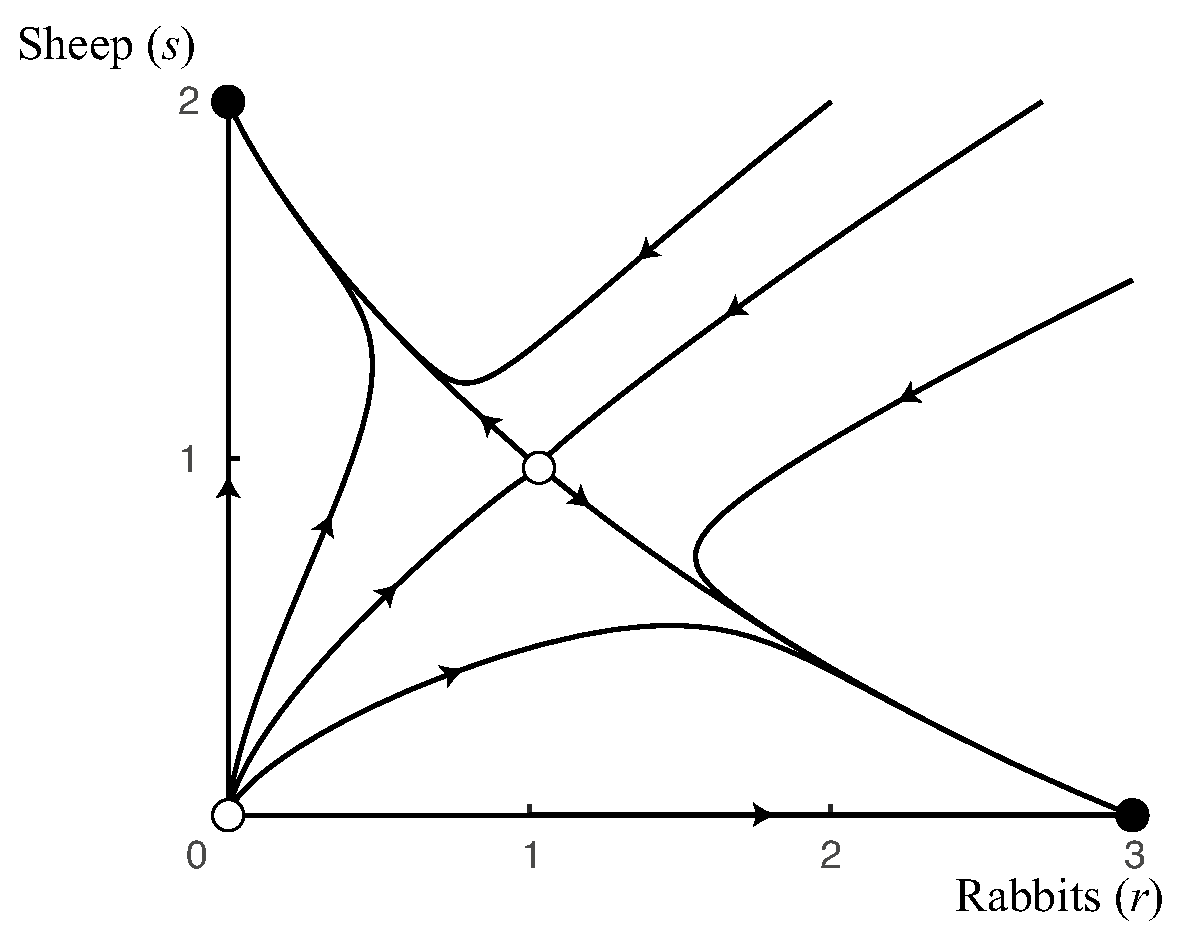
\includegraphics[width=0.55\textwidth]{Images/lotka-volterra.eps}
    \caption{Sample figure.}
 \label{sample-figure-1}
\end{figure}





\chapter{Theoretical background}
\label{background-chapter}

\section{Some equations}


\begin{align}
  &\begin{aligned}
E(u,v)   = & \int \int  t(x,y) e^{-2 \pi i (ux + vy)} \mathrm{d}x \mathrm{d}y\\
= & \sum_{n=0}^{N-1} \sum_{m=0}^{M-1}  \int_{-b + 2bm}^{b + 2bm} \int_{cn - a/2 + |y - 2m|\tan \theta}^{cn + a/2 + |y - 2m|\tan \theta} e^{-2 \pi i (ux + vy)} \mathrm{d}x \mathrm{d}y.
  \end{aligned}
\end{align}


\begin{equation} t(x) = 
\begin{cases}
\alpha \quad n \gamma < x < n \gamma + \frac{\gamma - \epsilon}{2},\\
1   \quad n\gamma + \frac{\gamma - \epsilon}{2} < x < n \gamma +  \frac{\gamma + \epsilon}{2},\\
\alpha \quad n \gamma +  \frac{\gamma + \epsilon}{2} < x < (n+1) \gamma,\\
\end{cases}
\label{t-cases}
\end{equation}


%%%%%%%%%%%%%%%%%%%%%%%%%%%%%%%%%%%%%%%%%%%%%%%%%%%%%%%






\cleardoublepage
\phantomsection
\addcontentsline{toc}{chapter}{Bibliography}
\bibliographystyle{plain}
\bibliography{AllMyReferences}




\appendix
\chapter{T�tulo ap�ndice A}
\label{appendix-A}

 
\subsubsection{Publication details:}

\begin{itemize}

\item Title:

\item Authors:

\item Publication date: 

\item Published in 

\item DOI:

\end{itemize}




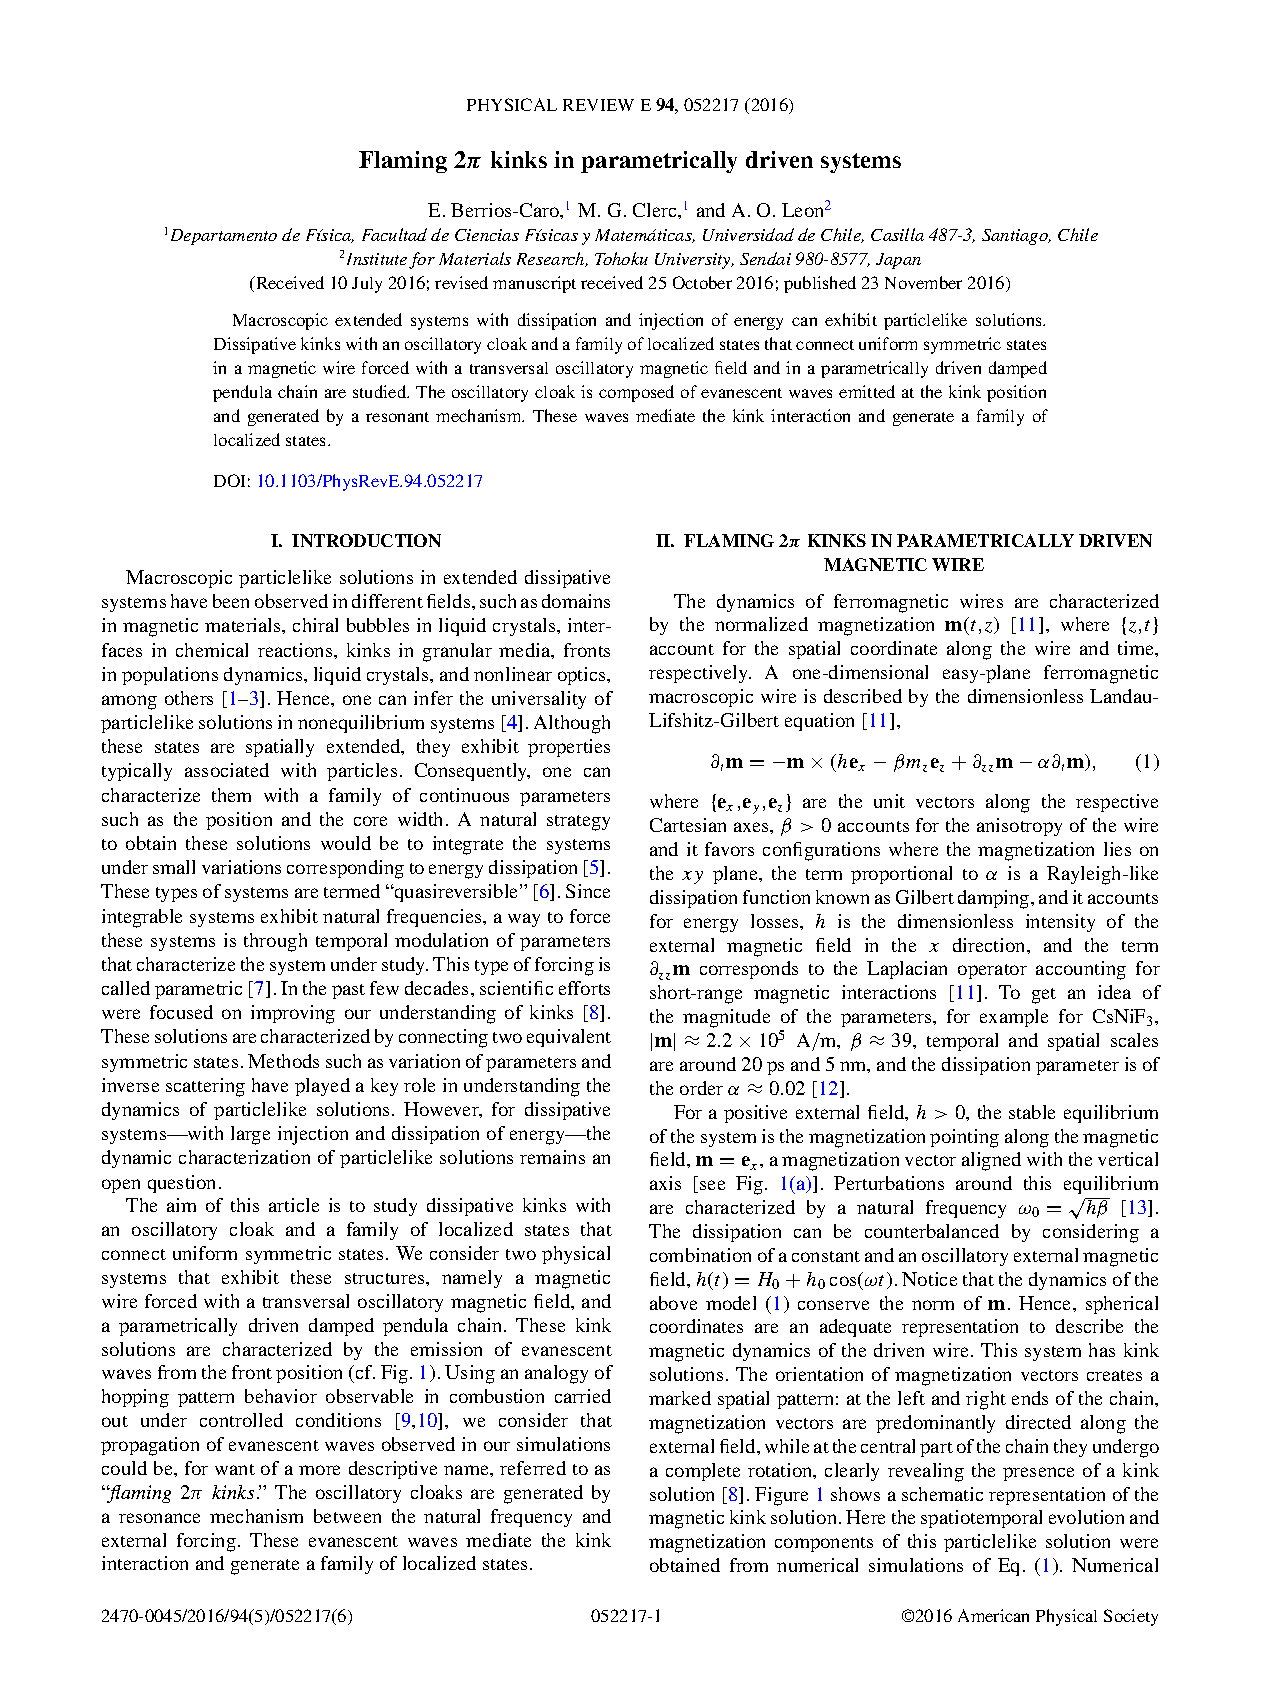
\includepdf[pages={1-6}]{Papers/Flamingkinkspaper.pdf}









\newpage

\end{document}
